\section{CAPÍTULO II: Marco contextual}

\subsection{Descripción del entorno de aplicación}

El proyecto se enfoca en contextos educativos secundarios, institucionales y universitarios donde los estudiantes han desarrollado patrones de comportamiento académico caracterizados por la búsqueda de aprobación sin compromiso real con el conocimiento \cite{academic_shortcuts2023,bretag2019}. A través de mecánicas de juego, progresión de habilidades y experiencias inmersivas en un entorno virtual medieval, la plataforma busca generar motivación intrínseca hacia el aprendizaje y revertir la percepción de irrelevancia que los estudiantes tienen sobre las tareas académicas.

\subsubsection{Gamificación Educativa}

La gamificación se define como la destreza de obtener elementos atractivos que se encuentran típicamente en los juegos y aplicarlos cuidadosamente en actividades productivas o del mundo real \cite{deterding2011}. Esta técnica ha ganado relevancia en diversos campos como la educación, el marketing y los entornos laborales, debido a su capacidad de fomentar la motivación, el compromiso y la participación activa.

El presente estudio explora qué hace atractivos a los juegos, resaltando aspectos como recompensas, diversión, interactividad, narrativa o historia, competencia, superación de retos y desafíos y posibilidad de compartir con amigos. Estos elementos, al ser incorporados estratégicamente en entornos no lúdicos, contribuyen a mejorar la experiencia del usuario y alcanzar objetivos específicos.

Contrario a lo que se podría pensar, las técnicas de gamificación no son recientes. Ya en el Imperio Romano existía un sistema de recompensas militares denominado Dona Militaria, el cual otorgaba distinciones como la Corona Cívica, por salvar la vida de un ciudadano, o la Corona Muralis, entregada al primer soldado que escalaba las murallas de una fortaleza enemiga, a pesar del alto riesgo de muerte \cite{polybius_histories}. Estos sistemas evidencian la existencia temprana de elementos como: feedback, insignias, competencia, colaboración, metas, niveles e interacción social.

Para comprender la gamificación en profundidad, es necesario distinguir entre los conceptos de juego y jugar. Jugar (Paidia) es una actividad espontánea, libre, sin finalidad concreta. Se asocia a la expresión creativa y la libertad de acción. Mientras que, Juego (Ludus): Actividad estructurada, con objetivos claros y reglas definidas. Implica una actitud deliberada de participación \cite{huizinga1938,caillois1961}.

La llamada actitud lúdica, conceptualizada por Friedrich Schiller \cite{schiller1795}, implica que los participantes se adhieren voluntariamente a las reglas del juego, le otorgan significado y están dispuestos a superar obstáculos innecesarios. En la gamificación, el desafío es lograr que el participante se acerque lo más posible al llamado "Círculo Mágico" del juego, donde se produce una inmersión total y significativa que potencia la motivación y la respuesta positiva ante los incentivos.

\paragraph{Modelo de Elementos de Gamificación}
Uno de los modelos más representativos para estructurar los elementos de la gamificación es la Pirámide de elementos \cite{werbach2012}, la cual se compone de tres niveles:

\begin{itemize}
\item \textbf{Dinámicas}: Son factores de diseño fundamentales relacionados con la naturaleza humana, como estatus, recompensa, competencia, altruismo, logro, emoción, progresión, relaciones y narrativa. Son universales e independientes del contexto cultural o demográfico.
\item \textbf{Mecánicas}: Son las reglas y sistemas que guían las acciones dentro de la experiencia gamificada, promoviendo el disfrute y el compromiso. Incluyen restricciones, desafíos, cooperación, retroalimentación y estrategias de progresión.
\item \textbf{Componentes}: Son elementos concretos y visibles, tales como logros, avatares, insignias, tablas de posiciones, puntos, equipos, niveles, objetos virtuales, recompensas y contenido desbloqueable.
\end{itemize}

\paragraph{Tipología de Jugadores}
Richard Bartle \cite{bartle1996} propuso una tipología de jugadores según su orientación hacia la acción o la interacción, y según el foco en el entorno o en los demás:

\begin{itemize}
\item \textbf{Triunfadores}: Están enfocados en progresar y dominar el entorno.
\item \textbf{Asesinos}: Buscan competir o dominar a otros jugadores.
\item \textbf{Exploradores}: Interesados en descubrir y comprender el mundo del juego.
\item \textbf{Socializadores}: Disfrutan de la interacción con otros participantes.
\end{itemize}

\paragraph{Misión}
Transformar las herramientas digitales de atajos académicos en facilitadores genuinos del aprendizaje mediante una plataforma 3D inmersiva que gamifica el proceso de enseñanza-aprendizaje, generando motivación intrínseca hacia el conocimiento y revertiendo patrones de comportamiento académico superficial a través de un mundo virtual medieval que convierte las tareas educativas en experiencias de aprendizaje significativas.

\paragraph{Visión}
Ser la plataforma educativa 3D de referencia mundial que establezca un nuevo paradigma en la relación entre estudiantes, herramientas digitales y conocimiento, donde el proceso de aprender sea tan atractivo y rewarding como obtener la calificación final, transformando definitivamente el uso de la tecnología en contextos educativos.

\paragraph{Análisis FODA}
El análisis FODA identifica las fortalezas, oportunidades, debilidades y amenazas del proyecto de gamificación educativa, proporcionando una base estratégica para la toma de decisiones en el desarrollo e implementación de la solución.

\begin{figure}[H]
	\centering
	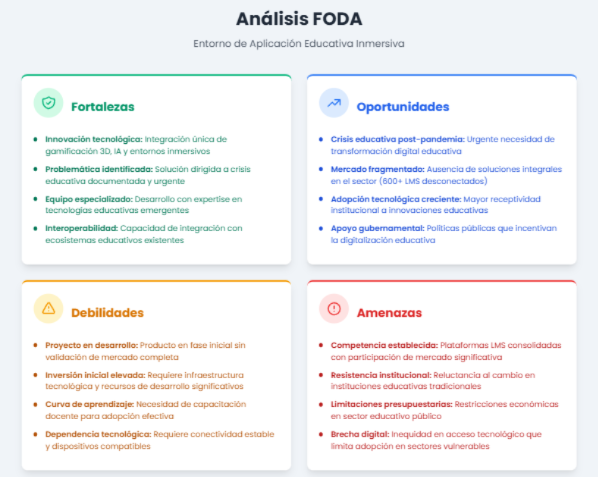
\includegraphics[width=0.9\textwidth]{images/analisis_foda.png}
	\caption{Análisis FODA del proyecto.}
	\label{fig:foda}
\end{figure}

\subsection{Fundamentos teóricos}

\subsubsection{Metodología de desarrollo de Software}

Una metodología para el desarrollo de software es un marco de trabajo que se usa para estructurar, planificar y controlar el proceso de desarrollo de sistemas de información \cite{velneo2023}.

\paragraph{Enfoque Ágil}
Las metodologías ágiles proporcionan una serie de pautas y principios junto a técnicas pragmáticas que hacen que la entrega del proyecto sea menos complicada y más satisfactoria tanto para los clientes como para los equipos de trabajo \cite{mayda2015}.

\myparagraph{Metodología Kanban}
La metodología Kanban es un marco ágil de flujo continuo que facilita la gestión visual del trabajo mediante un tablero y límites de trabajo en curso (WIP). Es especialmente adecuado para equipos pequeños y con disponibilidad limitada, ya que minimiza ceremonias formales y permite adaptar el flujo de trabajo a la capacidad real del equipo \cite{anderson2010}.

\subsubsection{Tecnologías de Desarrollo 3D}

\paragraph{Motores de renderizado 3D}
Los motores de renderizado 3D son frameworks que permiten crear, manipular y visualizar contenido tridimensional en aplicaciones web y móviles.

\myparagraph{Three.js}
Three.js es una biblioteca de JavaScript que abstrae WebGL para crear y renderizar escenas 3D con geometrías, materiales, luces y cámaras \cite{threejs2023}.

\myparagraph{Unity WebGL}
Unity WebGL es una plataforma de desarrollo que permite exportar aplicaciones Unity para ejecutarse en navegadores web mediante WebAssembly \cite{unity2023}.

\myparagraph{Babylon.js}
Babylon.js es un motor 3D en tiempo real desarrollado por Microsoft que se ejecuta en navegadores web usando WebGL y WebXR \cite{microsoft2023}.

\subsubsection{Frameworks de Desarrollo Backend}

\paragraph{Node.js}
Node.js es un entorno de tiempo de ejecución de JavaScript open source y multiplataforma que se ejecuta del lado del servidor. Utiliza un modelo basado en eventos asíncronos que permite gestionar múltiples conexiones simultáneas de forma eficiente \cite{acibeiro2022}, ideal para manejar las interacciones en tiempo real del entorno gamificado.

\paragraph{Next.js (API routes)}
Next.js es el framework elegido para integrar frontend y backend en una sola aplicación \cite{nextjs_docs2024}. Mediante las API routes de Next.js (con TypeScript) se implementarán endpoints server-side que gestionan autenticación, lógica de misiones, evaluación y acceso a la base de datos. Esta aproximación simplifica el despliegue y el mantenimiento al unificar el repositorio, aprovechar ventajas de SSR/SSG y facilitar la integración entre la parte UI (React/Three.js) y la capa de datos.

\paragraph{Django}
Django es un framework de desarrollo para Python que se emplea para la creación de páginas web. Se trata de una herramienta de código abierto que facilita el desarrollo web mediante su arquitectura Model-View-Template \cite{fernandez2022}, proporcionando robustez para el manejo de datos educativos y perfiles de usuario.

\subsubsection{Frameworks de Desarrollo Frontend}

\paragraph{React}
ReactJS es una biblioteca de JavaScript para el desarrollo de aplicaciones móviles y web. Contiene una colección de fragmentos de código JavaScript reutilizables utilizados para crear interfaces de usuario llamadas componentes \cite{deyimar2023}, facilitando la creación de interfaces interactivas para la gestión de tareas gamificadas.

\paragraph{Vue.js}
Vue.js es un framework open source de JavaScript que permite construir interfaces de usuarios de forma sencilla. Su característica principal es el trabajo con componentes reutilizables \cite{garcia2019}, ideal para desarrollar paneles de control y dashboards de progreso estudiantil.

\paragraph{Angular}
Angular es un framework front-end desarrollado por Google, diseñado para la creación de aplicaciones web robustas y escalables. Utiliza TypeScript y se basa en una arquitectura de componentes \cite{roldan2020}, proporcionando estructura sólida para aplicaciones educativas complejas.

\paragraph{Next.js}
Next.js es un framework construido sobre React que facilita el renderizado híbrido (SSR/SSG), generación de páginas estáticas y enrutamiento automático \cite{nextjs_docs2024}. Ofrece optimizaciones de rendimiento, manejo de rutas y capacidades de API que son útiles para construir portales educativos, dashboards y páginas con requisitos SEO y carga rápida sin sacrificar la interactividad del frontend.

\paragraph{Expo}
Expo es una plataforma y conjunto de herramientas para desarrollar aplicaciones móviles con React Native de forma rápida y con menos configuración \cite{expo_docs2023}. Permite prototipado ágil, despliegues OTA (over-the-air) y compatibilidad con Expo Go para pruebas en dispositivos reales, lo que facilita construir versiones móviles de la plataforma educativa para estudiantes y docentes.

\subsubsection{Sistemas de Base de Datos}

\paragraph{PostgreSQL}
PostgreSQL es un sistema de gestión de bases de datos relacional de código abierto que proporciona soporte para transacciones ACID, escalabilidad y extensibilidad. Ofrece características avanzadas como procedimientos almacenados y tipos de datos personalizados \cite{postgresql2024}, ideal para mantener la integridad de los datos educativos y el progreso estudiantil.

\paragraph{MongoDB}
MongoDB es una base de datos NoSQL orientada a documentos que almacena datos en formato JSON-like (BSON). Es especialmente útil para aplicaciones que requieren flexibilidad en el esquema de datos y escalabilidad horizontal \cite{mongodb2023}, permitiendo almacenar configuraciones dinámicas de misiones y logros estudiantiles.

\subsubsection{ORM}
\paragraph{Prisma}
Prisma es una opción  para interactuar con PostgreSQL desde las API routes de Next.js \cite{prisma_docs2024}. Ofrece tipado fuerte (TypeScript), generación automática de cliente, migraciones controladas y una DX (developer experience) que acelera el desarrollo. Prisma facilita modelar entidades como Usuarios, Misiones, Evaluaciones y Progreso y se integra bien con pruebas y despliegues.

\paragraph{Sequelize}
Sequelize es un ORM maduro para Node.js que soporta múltiples bases de datos SQL \cite{sequelize_docs2023}. Proporciona un API flexible, asociaciones explícitas y migraciones. Es una opción viable cuando se requiere compatibilidad con proyectos existentes en JavaScript puro o cuando se necesita un control granular de las consultas SQL.

\paragraph{TypeORM}
TypeORM es un ORM orientado a TypeScript que ofrece un enfoque tradicional basado en decoradores y entidades \cite{typeorm_docs2022}. Es útil en proyectos que prefieren una capa de abstracción con sintaxis declarativa y tiene buen soporte para patrones DDD (Domain-Driven Design). Sin embargo, su performance y DX pueden ser menos modernas que las de Prisma en ciertos flujos de trabajo.

\subsubsection{Plataformas de Despliegue}

\paragraph{Docker}
Docker es una plataforma de contenerización que empaqueta aplicaciones y sus dependencias en contenedores ligeros, garantizando portabilidad y consistencia entre entornos de desarrollo, pruebas y producción \cite{docker2023}. Facilita el despliegue de la aplicación educativa en diferentes instituciones.

\paragraph{Kubernetes}
Kubernetes es una plataforma de orquestación de contenedores que automatiza el despliegue, escalado y gestión de aplicaciones contenerizadas, proporcionando alta disponibilidad y recuperación automática \cite{kubernetes2023}. Permite manejar múltiples instancias concurrentes del entorno virtual para diferentes instituciones educativas.

\subsection{2.3 Descripción de los interesados del proyecto}

Los principales interesados del proyecto incluyen:

\begin{itemize}
	\item \textbf{Estudiantes}: Usuarios finales que interactuarán con la plataforma gamificada. Son el grupo objetivo principal y su adopción determinará el impacto pedagógico.
	\item \textbf{Docentes}: Creadores de contenido y evaluadores del proceso educativo. Diseñan las tareas, evalúan el rendimiento y configuran mecánicas y recompensas.
	\item \textbf{Instituciones educativas}: Adoptantes de la solución tecnológica. Se encargan de la implementación organizacional, políticas y financiamiento.
	\item \textbf{Área de TI}: Responsables de la implementación y mantenimiento técnico, despliegue en contenedores, monitoreo y backups.
	\item \textbf{Organismos reguladores}: Entidades que supervisan el cumplimiento de estándares educativos, privacidad y protección de datos.
\end{itemize}

\subsection{2.4 Análisis de la solución}

\subsubsection{2.4.1 Evaluación de motores de renderizado 3D}
Para el desarrollo del entorno 3D inmersivo se evalúan tres alternativas: Three.js, Unity WebGL y Babylon.js. Se empleará el método Scoring \cite{belton2002} para determinar la mejor opción. Este método de análisis multicriterio permite evaluar alternativas asignando ponderaciones a criterios relevantes y puntuaciones de satisfacción a cada opción, calculando un puntaje total que facilita la toma de decisiones objetivas.

\paragraph{Objetivo}
Seleccionar la mejor herramienta para el desarrollo del entorno 3D.

\paragraph{Alternativas}
Three.js, Unity WebGL, Babylon.js.

\paragraph{Criterios de evaluación}
Facilidad de uso, rendimiento, compatibilidad web, soporte de comunidad.
% A continuación se muestran las tablas de ponderación y satisfacción para la evaluación de motores 3D:
% Tabla 1
\begin{table}[ht]
\centering
\caption{Ponderación de los criterios motores de renderizado 3D (Valores asignados por el autor siguiendo metodología Scoring; ver \cite{belton2002})}
\begin{tabular}{l c}
\hline
Criterios & Ponderación \\
\hline
Facilidad de uso & 4 \\
Rendimiento & 5 \\
Compatibilidad web & 5 \\
Soporte de comunidad & 4 \\
\hline
\end{tabular}
\end{table}

% Tabla 2
\begin{table}[ht]
\centering
\caption{Nivel de satisfacción motores de renderizado 3D (Estimaciones del autor basadas en documentación técnica)}
\begin{tabular}{l c c c}
\hline
Criterios & Three.js & Unity WebGL & Babylon.js \\
\hline
Facilidad de uso & 8 & 6 & 7 \\
Rendimiento & 7 & 9 & 8 \\
Compatibilidad web & 9 & 7 & 8 \\
Soporte de comunidad & 9 & 8 & 6 \\
\hline
\end{tabular}
\end{table}
\FloatBarrier

% Tabla 3
\begin{table}[ht]
\centering
\caption{Comparación de motores de renderizado 3D}
\begin{tabular}{l c c c c}
\hline
Criterios & Ponderación & Three.js & Unity WebGL & Babylon.js \\
\hline
Facilidad de uso & 4 & 8 & 6 & 7 \\
Rendimiento & 5 & 7 & 9 & 8 \\
Compatibilidad web & 5 & 9 & 7 & 8 \\
Soporte de comunidad & 4 & 9 & 8 & 6 \\
\hline
Puntaje & - & 148 & 134 & 139 \\
\hline
\end{tabular}
\end{table}
\FloatBarrier
% --- Resultado para motores 3D (colocado después de sus tablas) ---
\subsubsection{2.4.1.1 Resultado de análisis de motores de renderizado 3D}
Considerando los resultados del método Scoring \cite{belton2002}, Three.js \cite{threejs2023} es la mejor opción para el desarrollo del entorno 3D debido a su excelente compatibilidad web, amplio soporte de comunidad y facilidad de integración con tecnologías web estándar.

% --- Evaluación de frameworks backend (descripción antes de tablas) ---
\subsubsection{2.4.2 Evaluación de frameworks backend}
Se evalúan tres frameworks para el desarrollo del backend: Node.js con NestJS, Django y Express.js.

\paragraph{Criterios de evaluación}
Escalabilidad, facilidad de desarrollo, rendimiento, ecosistema.
% A continuación se muestran las tablas de ponderación y satisfacción para la evaluación de frameworks backend:
% Tabla 4
\begin{table}[ht]
\centering
\caption{Ponderación de los criterios frameworks backend (Valores asignados por el autor siguiendo metodología Scoring; ver \cite{belton2002})}
\begin{tabular}{l c}
\hline
Criterios & Ponderación \\
\hline
Escalabilidad & 5 \\
Facilidad de desarrollo & 4 \\
Rendimiento & 5 \\
Ecosistema & 4 \\
\hline
\end{tabular}
\end{table}
\FloatBarrier

% Tabla 5
\begin{table}[ht]
\centering
\caption{Nivel de satisfacción frameworks backend (Estimaciones del autor basadas en documentación técnica)}
\begin{tabular}{l c c c}
\hline
Criterios & NestJS & Django & Express.js \\
\hline
Escalabilidad & 9 & 7 & 6 \\
Facilidad de desarrollo & 8 & 9 & 7 \\
Rendimiento & 8 & 6 & 8 \\
Ecosistema & 8 & 8 & 9 \\
\hline
\end{tabular}
\end{table}
\FloatBarrier

% Tabla 6
\begin{table}[ht]
\centering
\caption{Comparación de frameworks backend}
\begin{tabular}{l c c c c}
\hline
Criterios & Ponderación & NestJS & Django & Express.js \\
\hline
Escalabilidad & 5 & 9 & 7 & 6 \\
Facilidad de desarrollo & 4 & 8 & 9 & 7 \\
Rendimiento & 5 & 8 & 6 & 8 \\
Ecosistema & 4 & 8 & 8 & 9 \\
\hline
Puntaje & - & 149 & 126 & 132 \\
\hline
\end{tabular}
\end{table}
\FloatBarrier
% --- Resultado para frameworks backend (colocado después de sus tablas) ---
\subsubsection{2.4.2.1 Resultado de análisis de frameworks backend}
NestJS obtiene la mejor puntuación debido a su arquitectura modular, excelente escalabilidad y integración nativa con TypeScript, lo que facilita el desarrollo de APIs robustas para la aplicación educativa.

% --- Evaluación de frameworks frontend (descripción antes de tablas) ---
\subsubsection{2.4.3 Evaluación de frameworks frontend}
Se evalúan tres frameworks (y alternativas relacionadas) para el desarrollo del frontend: React, Vue.js, Angular, Next.js y Expo.

\paragraph{Criterios de evaluación}
Curva de aprendizaje, rendimiento, ecosistema, integración 3D.
% A continuación se muestran las tablas de ponderación y satisfacción para la evaluación de frameworks frontend:
% Tabla 7
\begin{table}[ht]
\centering
\caption{Ponderación de los criterios frameworks frontend (Valores asignados por el autor siguiendo metodología Scoring; ver \cite{belton2002})}
\begin{tabular}{l c}
\hline
Criterios & Ponderación \\
\hline
Curva de aprendizaje & 4 \\
Rendimiento & 5 \\
Ecosistema & 4 \\
Integración 3D & 5 \\
\hline
\end{tabular}
\end{table}
\FloatBarrier

% Tabla 8
\begin{table}[ht]
\centering
\caption{Nivel de satisfacción frameworks frontend (Estimaciones del autor basadas en documentación técnica)}
\begin{tabular}{l c c c c c}
\hline
Criterios & React & Vue.js & Angular & Next.js & Expo \\
\hline
Curva de aprendizaje & 7 & 9 & 5 & 7 & 8 \\
Rendimiento & 8 & 8 & 7 & 9 & 6 \\
Ecosistema & 9 & 7 & 8 & 9 & 6 \\
Integración 3D & 9 & 6 & 7 & 9 & 5 \\
\hline
\end{tabular}
\end{table}
\FloatBarrier

% Tabla 9
\begin{table}[ht]
\centering
\caption{Comparación de frameworks frontend}
\begin{tabular}{l c c c c c c}
\hline
Criterios & Ponderación & React & Vue.js & Angular & Next.js & Expo \\
\hline
Curva de aprendizaje & 4 & 7 & 9 & 5 & 6 & 8 \\
Rendimiento & 5 & 8 & 8 & 7 & 9 & 6 \\
Ecosistema & 4 & 9 & 7 & 8 & 8 & 6 \\
Integración 3D & 5 & 9 & 6 & 7 & 9 & 5 \\
\hline
Puntaje & - & 149 & 134 & 122 & 154 & 111 \\
\hline
\end{tabular}
\end{table}
\FloatBarrier
% --- Resultado para frameworks frontend (colocado después de sus tablas) ---
\subsubsection{2.4.3.1 Resultado de análisis de frameworks frontend}
Según los resultados del análisis multicriterio \cite{belton2002}, Next.js \cite{nextjs_docs2024} es la opción recomendada para el frontend en este proyecto debido a su excelente integración con bibliotecas 3D (cuando se usa junto a React/Three.js), sus capacidades de renderizado híbrido (SSR/SSG), y sus optimizaciones de rendimiento para páginas con requisitos SEO y cargas iniciales rápidas. React sigue siendo una opción sólida y más generalista, pero en función de los criterios y ponderaciones utilizadas, Next.js obtiene el puntaje más alto. Expo \cite{expo_docs2023} mantiene utilidad para prototipado y versiones móviles, pero queda por detrás en la integración 3D.

% --- Evaluación de sistemas de base de datos (descripción antes de tablas) ---
\subsubsection{2.4.4 Evaluación de sistemas de base de datos}
Se evalúan dos sistemas de base de datos: PostgreSQL y MongoDB.

\paragraph{Criterios de evaluación}
Consistencia de datos, escalabilidad, facilidad de uso, soporte.
% A continuación se muestran las tablas de ponderación y satisfacción para la evaluación de sistemas de base de datos:
% Tabla 10
\begin{table}[ht]
\centering
\caption{Ponderación de los criterios sistemas de base de datos (Valores asignados por el autor siguiendo metodología Scoring; ver \cite{belton2002})}
\begin{tabular}{l c}
\hline
Criterios & Ponderación \\
\hline
Consistencia de datos & 5 \\
Escalabilidad & 4 \\
Facilidad de uso & 4 \\
Soporte & 3 \\
\hline
\end{tabular}
\end{table}

% Tabla 11
\begin{table}[ht]
\centering
\caption{Nivel de satisfacción sistemas de base de datos (Estimaciones del autor basadas en documentación técnica)}
\begin{tabular}{l c c}
\hline
Criterios & PostgreSQL & MongoDB \\
\hline
Consistencia de datos & 9 & 6 \\
Escalabilidad & 7 & 9 \\
Facilidad de uso & 7 & 8 \\
Soporte & 9 & 7 \\
\hline
\end{tabular}
\end{table}

% Tabla 12
\begin{table}[ht]
\centering
\caption{Comparación de sistemas de base de datos}
\begin{tabular}{l c c c}
\hline
Criterios & Ponderación & PostgreSQL & MongoDB \\
\hline
Consistencia de datos & 5 & 9 & 6 \\
Escalabilidad & 4 & 7 & 9 \\
Facilidad de uso & 4 & 7 & 8 \\
Soporte & 3 & 9 & 7 \\
\hline
Puntaje & - & 134 & 118 \\
\hline
\end{tabular}
\end{table}

\subsubsection{2.4.4.1 Resultado de análisis de sistemas de base de datos}
PostgreSQL es la mejor opción debido a su robustez, consistencia de datos mediante transacciones ACID y excelente soporte para datos relacionales complejos necesarios en un sistema educativo.

% --- Evaluación de ORMs (descripción antes de tablas) ---
\subsubsection{2.4.5 Evaluación de ORM}
Se evalúan tres ORMs populares para integrar la capa de datos con las API routes de Next.js: Prisma, Sequelize y TypeORM. Se aplicará nuevamente el método Scoring \cite{belton2002} para comparar alternativas según criterios relevantes para este proyecto.

\paragraph{Criterios de evaluación}
Tipado/seguridad, facilidad de uso, rendimiento, migraciones y experiencia de desarrollador (DX).
% A continuación se muestran las tablas de ponderación y satisfacción para la evaluación de ORMs:
% Tabla 13
\begin{table}[ht]
\centering
\caption{Ponderación de los criterios ORMs (Valores asignados por el autor siguiendo metodología Scoring; ver \cite{belton2002})}
\begin{tabular}{l c}
\hline
Criterios & Ponderación \\
\hline
Tipado / Seguridad & 5 \\
Facilidad de uso & 4 \\
Rendimiento & 4 \\
Migraciones & 3 \\
Experiencia de desarrollador (DX) & 4 \\
\hline
\end{tabular}
\end{table}
\FloatBarrier

% Tabla 14
\begin{table}[ht]
\centering
\caption{Nivel de satisfacción ORMs (Estimaciones del autor basadas en documentación técnica)}
\begin{tabular}{l c c c}
\hline
Criterios & Prisma & Sequelize & TypeORM \\
\hline
Tipado / Seguridad & 9 & 6 & 8 \\
Facilidad de uso & 8 & 7 & 7 \\
Rendimiento & 8 & 7 & 7 \\
Migraciones & 8 & 7 & 6 \\
DX & 9 & 7 & 7 \\
\hline
\end{tabular}
\end{table}
\FloatBarrier

% Tabla 15
\begin{table}[ht]
\centering
\caption{Comparación de ORMs}
\begin{tabular}{l c c c c}
\hline
Criterios & Ponderación & Prisma & Sequelize & TypeORM \\
\hline
Tipado / Seguridad & 5 & 9 & 6 & 8 \\
Facilidad de uso & 4 & 8 & 7 & 7 \\
Rendimiento & 4 & 8 & 7 & 7 \\
Migraciones & 3 & 8 & 7 & 6 \\
DX & 4 & 9 & 7 & 7 \\
\hline
Puntaje & - &  \textendash &  \textendash &  \textendash \\
\hline
\end{tabular}
\end{table}
\FloatBarrier

% Calcular puntaje total (mostrado en texto para mantener el control en LaTeX)
\subsubsection{2.4.5.1 Resultado de análisis de ORMs}
Aplicando la matriz de ponderaciones y multiplicando por las puntuaciones de satisfacción (cada criterio sobre 10), se obtiene un puntaje aproximado (redondeado) que favorece a Prisma en este contexto de Next.js con TypeScript debido a su tipado fuerte, excelente DX y sistema de migraciones integrado \cite{prisma_docs2024,sequelize_docs2023,typeorm_docs2022}. Por tanto, se recomienda adoptar Prisma como ORM principal para la implementación de las API routes y la gestión de entidades como Usuarios, Misiones y Progreso.

\paragraph{Observaciones}
Prisma ofrece ventajas significativas en proyectos TypeScript por su cliente tipado, generación de tipos y migraciones declarativas. Sequelize sigue siendo una opción válida si se requiere compatibilidad con código JavaScript existente, mientras que TypeORM puede ser preferible en equipos que favorezcan un estilo declarativo con decoradores y entidades al estilo tradicional \cite{prisma_docs2024,sequelize_docs2023,typeorm_docs2022}.


